% Template for Cogsci submission with R Markdown

% Stuff changed from original Markdown PLOS Template
\documentclass[10pt, letterpaper]{article}

\usepackage{cogsci}
\usepackage{pslatex}
\usepackage{float}
\usepackage{caption}

% amsmath package, useful for mathematical formulas
\usepackage{amsmath}

% amssymb package, useful for mathematical symbols
\usepackage{amssymb}

% hyperref package, useful for hyperlinks
\usepackage{hyperref}

% graphicx package, useful for including eps and pdf graphics
% include graphics with the command \includegraphics
\usepackage{graphicx}

% Sweave(-like)
\usepackage{fancyvrb}
\DefineVerbatimEnvironment{Sinput}{Verbatim}{fontshape=sl}
\DefineVerbatimEnvironment{Soutput}{Verbatim}{}
\DefineVerbatimEnvironment{Scode}{Verbatim}{fontshape=sl}
\newenvironment{Schunk}{}{}
\DefineVerbatimEnvironment{Code}{Verbatim}{}
\DefineVerbatimEnvironment{CodeInput}{Verbatim}{fontshape=sl}
\DefineVerbatimEnvironment{CodeOutput}{Verbatim}{}
\newenvironment{CodeChunk}{}{}

% cite package, to clean up citations in the main text. Do not remove.
\usepackage{apacite}

% KM added 1/4/18 to allow control of blind submission


\usepackage{color}

% Use doublespacing - comment out for single spacing
%\usepackage{setspace}
%\doublespacing


% % Text layout
% \topmargin 0.0cm
% \oddsidemargin 0.5cm
% \evensidemargin 0.5cm
% \textwidth 16cm
% \textheight 21cm

\title{How to Make a Proceedings Paper Submission}


\author{{\large \bf Morton Ann Gernsbacher (MAG@Macc.Wisc.Edu)} \\ Department of Psychology, 1202 W. Johnson Street \\ Madison, WI 53706 USA \AND {\large \bf Sharon J.~Derry (SDJ@Macc.Wisc.Edu)} \\ Department of Educational Psychology, 1025 W. Johnson Street \\ Madison, WI 53706 USA}


\begin{document}

\maketitle

\begin{abstract}
Include no author information in the initial submission, to facilitate
blind review. The abstract should be one paragraph, indented 1/8 inch on
both sides, in 9\textasciitilde point font with single spacing. The
heading `Abstract' should be 10\textasciitilde point, bold, centered,
with one line of space below it. This one-paragraph abstract section is
required only for standard six page proceedings papers. Following the
abstract should be a blank line, followed by the header `Keywords' and a
list of descriptive keywords separated by semicolons, all in
9\textasciitilde point font, as shown below.

\textbf{Keywords:}
Add your choice of indexing terms or keywords; kindly use a semi-colon;
between each term.
\end{abstract}

\hypertarget{introduction}{%
\section{Introduction}\label{introduction}}

\hypertarget{experiment-r-child-02_experiment.rmd}{%
\section{Experiment \{r child =
``02\_experiment.Rmd''\}}\label{experiment-r-child-02_experiment.rmd}}

\begin{verbatim}
\end{verbatim}

\hypertarget{model}{%
\section{Model}\label{model}}

We formalized the learning problem that participants face in our
experiments as a form of Bayesian concept learning (Tenenbaum, 1999;
Goodman, 2006), represented graphically in Fig. X. The goal is to learn
a concept \(theta\), which is a set of probabilities for independent
binary features \(\theta_{1,2,..,n}\), where n is the number of
features. Over the course of a block, the learner receives information
about \(\theta\) by observing exemplars \(y\): instantiations of
\(\bar{\theta}\), where each feature \(y_{1,2,..,n}\) is either on or
off. Each feature \(\theta_i\) and its corresponding exemplar \(y_i\)
form a Beta-Bernoulli process: \begin{eqnarray}
p(\theta_i) \sim Beta(\alpha_i,\beta_i) \\
p(y_i|\theta_i) \sim Bernoulli(\theta_i)
\end{eqnarray} Since the features are independent, this relationship
holds for the entire concept \(\theta\). However, to model the time
course of attention, we do not want to assume that information is
encoded perfectly and instantaneously. Instead, we suggest that
participants gather repeated noisy samples \(\bar{z}\) from the
exemplars. For any sample \(z\) from an exemplar \(y\) there is a small
probability \(\epsilon\) to misperceive the feature as off when it was
actually on, and vice versa. Therefore, by making noisy observations
\(\bar{z}\), the learner obtains information about the true identity of
the exemplar \(y\), and by extension, about the concept \(\bar{theta}\).
By Bayes' rule: \begin{eqnarray}
P(\theta|\bar{z}) &= p(\bar{z}|y) p(y|\theta) p(\theta) / p(\bar{z})
\end{eqnarray} where \(p(\bar{z}|y_i)\) is fully described by
\(\epsilon\), and \(p(y|\theta)\) by Bernoulli processes as in Eq. 2.

\begin{CodeChunk}
\begin{figure}[H]

{\centering 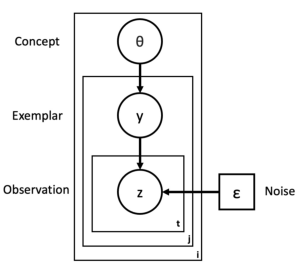
\includegraphics{figs/image-1} 

}

\caption[Graphical representation of our model]{Graphical representation of our model. Circles indicate random variables. The squares indicate fixed model parameters.}\label{fig:image}
\end{figure}
\end{CodeChunk}

Like in our experiment, the learner's task is to decide when to stop
sampling. If they do so rationally, then they should anchor their
sampling behavior to the expected information gain (EIG) of the next
sample. We compute EIG by weighing the information gain from each
possible next observation by the probability of that observation. We
defined information gain as the KL-divergence between the hypothetical
posterior after observing a sample \(z_{t+1}\) and the current
posterior: \begin{eqnarray}
EIG(z_{t+1}) = \sum_{z_{t+1} \in [0,1]} p(z_{t+1}|\theta_t) * KL(\theta_{t+1}, p(\theta_t))
\end{eqnarray} Finally, to get actual sampling behavior from the model,
it has to convert EIG into a binary decision about whether continue
looking at the current sample, or to advance to the next trial. The
model does so using a luce choice between the EIG from the next sample
and a constant EIG from looking away. \begin{eqnarray}
p(look) = \frac{EIG(z_{t+1})}{EIG(z_{t+1})+EIG(world)}
\end{eqnarray} We also studied the behavior of the model when replacing
EIG with other linking hypotheses, such as surprisal (the probability of
a given \(z\) under the \(P(\theta_t)\)) and KL-divergence between the
posterior \(p(\theta_t)\) and the prior \(p(\theta_{t-1})\).

\hypertarget{general-discussion}{%
\section{General Discussion}\label{general-discussion}}

\hypertarget{references}{%
\section{References}\label{references}}

\hypertarget{references-1}{%
\section{References}\label{references-1}}

\setlength{\parindent}{-0.1in} 
\setlength{\leftskip}{0.125in}

\noindent

\bibliographystyle{apacite}


\end{document}
